

%%% This LaTeX source document can be used as the basis for your technical
%%% report. Intentionally stripped and simplified
%%% and commands should be adjusted for your particular paper - title, 
%%% author, citations, equations, etc.
% % Citations/references are in report.bib 

\documentclass[conference,backref=page]{acmsiggraph}

\TOGonlineid{45678}
\TOGvolume{0}
\TOGnumber{0}
\TOGarticleDOI{1111111.2222222}
\TOGprojectURL{}
\TOGvideoURL{}
\TOGdataURL{}
\TOGcodeURL{}

% Include this so that citations show up in blue and the page information is included in the reference section
\hypersetup{
    colorlinks = true, 
    linkcolor = blue,
    anchorcolor = red,
    citecolor = blue, 
    filecolor = red, 
}


\title{Sky Wars\\
	  A Report on The Use of Patterns}

\author{Beej Persson \thanks{e-mail:40183743@live.napier.ac.uk} \\
Edinburgh Napier University\\
Software Development 3 (SET09101)}
\pdfauthor{Beej Persson}

\keywords{java, patterns, factory, strategy, observer, GUI, threads}

\begin{document}


\maketitle

\raggedbottom

\begin{abstract}

Sky Wars is a simple object-orientated game built using Java with particular attention paid to utilising specific programming design patterns and how to correctly implement them. The game has a working Graphical User Interface (GUI), use of threads and some triggered audio effects. This report looks to highlight the design patterns: where they were used and why, as well as discussing some of the main features of the GUI and how threads were used.

\end{abstract}



\keywordlist


\section{Patterns}


\subsection{Factory}
The factory pattern was used to create all the ships that are in the game; both enemies and the player. By using this pattern the factory class handled all creation of the ships, whilst the ship classes themselves only needed to indicate their ship type. Whilst the factory pattern's advantages tend to be in larger programs (a lot of classes are instantiated, unit-testability is simplified by unifying the tests into the factory class, and easy extensibility when adding new classes to be created), there are still benefits on a small program such as this game. If the factory pattern was not used, all the ships in the game would have to be initialised individually and a significant amount of extra and unnecessary code would be needed.

\subsection{Observer}
Initially the observer pattern was to be used to allow the ships (the observables) to pass their location data to the board (the observer) to be drawn in when running the game. Unfortunately this never seemed to work and as such a significantly simpler attempt to implement this pattern was made. The GUI's output text string would be observed by a class that simply displayed this text in the text box. However a working implementation of this was never found within the designated time-frame. This pattern would have helped enable more efficient communication between the initialised ship's locations and the board when drawing them.

\subsection{Strategy}
The benefit of the strategy pattern lies in separating certain algorithms into classes that can then be inserted at runtime. In this game the Master Ship had two operational modes: offensive and defensive. By storing the functionality of these modes inside classes that implement an operational mode interface the desired functionality of the Master Ship can be changed at runtime. This would also allow additional operational modes to be easily added later without having to override any methods.

\subsection{Command}
The command pattern is used to to instantiate methods by one class but run them sometime later by an invoker class. This pattern would be extremely useful in a turn based game such as this as the turns themselves could be instantiated and run separately allowing for comparatively simple ways of undoing a turn and reverting to a previous state. However, due to time constraints no implementation of this pattern was ever used in the game and as a direct result the 'Undo' button on the GUI has no function.


\section{Use of Threads}
For all the ships in the game a thread was created to handle it's attributes, such as location and type. This was done to more effectively track the ships whilst allowing ships to be added and removed without affecting the game state. Additionally if a way to undo moves had been implemented the stored information could be returned from then threads to help enable this.


\section{Graphical User Interface}
The Graphical User Interface was designed to be simple to use and simple to understand the state of the game. The GUI can be seen in Figure \ref{gui1}. The Sky grid has 16 squares with their coordinates labelled. The master ship spawns in and its position is displayed by showing its name in the square it's currently in. There are 5 buttons to control the game, 'Start', 'Move', 'Mode', 'Undo' and 'Quit', each with tool tips when the mouse is hovered over. On the right of the GUI is a text output field that displays the events of the game.

\begin{figure}[h]
	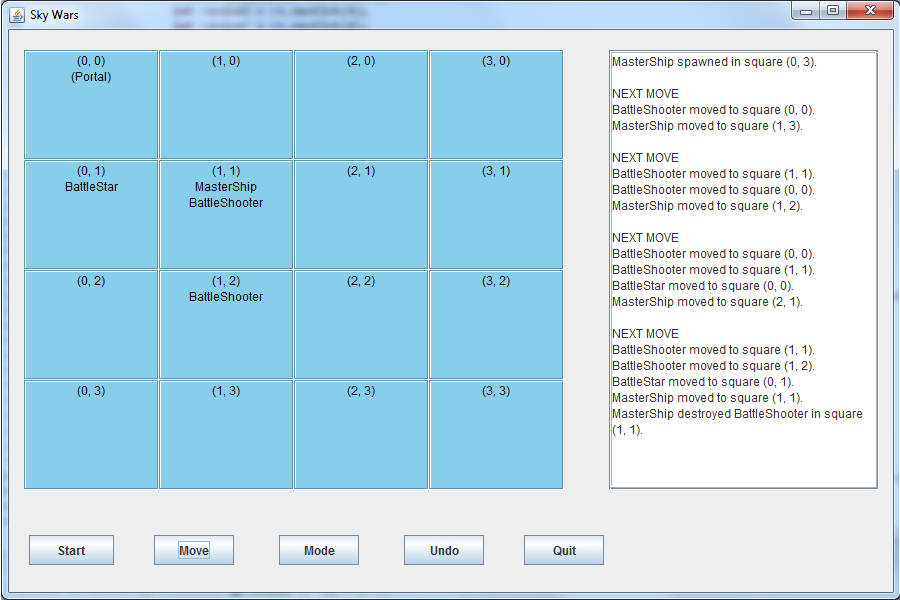
\includegraphics[width=\columnwidth]{images/gui1.png}
	\caption{An image showing the GUI when the game is running. There is a grid in which the ships move, buttons to control the game and a text output field displaying the events that have occurred.}
	\label{gui1}
\end{figure}

\begin{itemize}
	\item {\bf Start}: The 'Start' button starts the game and draws the board, spawning in the master ship but not enemies. If the game is running the 'Start' button will reset the game.
	\item {\bf Move}: The 'Move' button moves the master ship around the board. It also has a chance to spawn an enemy ship and once enemy ships have spawn it also moves those ships.
	\item {\bf Mode}: The 'Mode' button changes the master ship's operational mode between offensive and defensive and displays a message saying show as shown in Figure \ref{gui2}.
	\item {\bf Undo}: The 'Undo' button has no functionality at this current time. It was intended to return the state of the game to before the last time the 'Move' button was pressed, however was never implemented due to time constraints.
	\item {\bf Quit}: The 'Quit' button closes the game and the window.
	\item{\bf Output Field} The text output field was used to display information of events to the player, such as where the master ship has moved, when it kills enemy ships or is killed, and differentiating between which events happened in which turn.
\end{itemize}

\begin{figure}[h]
	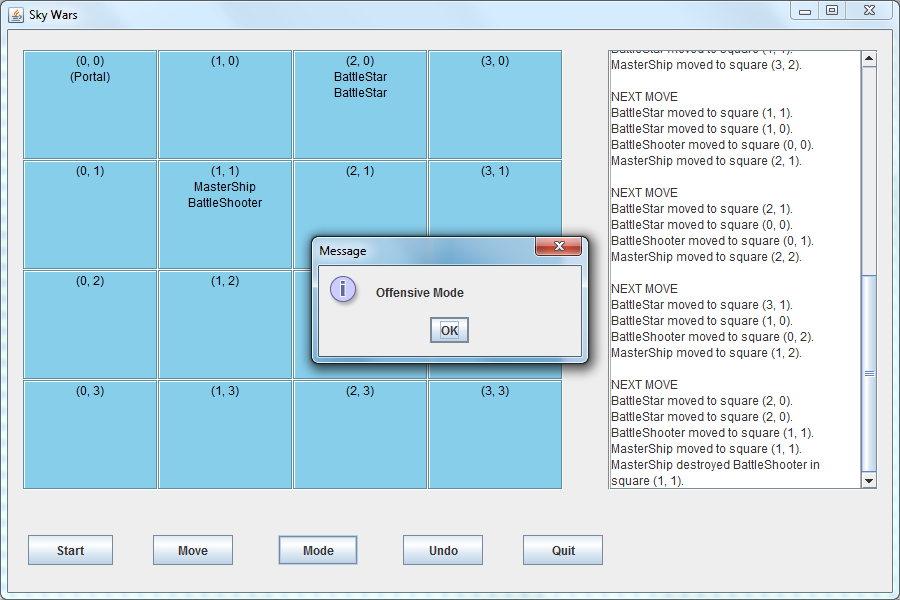
\includegraphics[width=\columnwidth]{images/gui2.png}
	\caption{An image showing the GUI when 'Mode' button is pressed, giving an indicator of the ship's current mode to the player.}
	\label{gui2}
\end{figure}

\section{Audio}
For this game there was a programming technique not taught in the module that was used. When the game is loaded there is music that runs when the 'Start' button is pressed. The music is initialised in its own class and multiple files can be stored in the project. The audio file can then be run at the desired time when the game is running by performing certain actions or as a result of events. There is also a sound that plays when the Master ship is destroyed to help provide more feedback to the player about their failure.

\section{Conclusion}
Sky Wars was a game created with the intention of exploring design patterns and their implementation in Java. This report has discussed the patterns used and attempted and how they benefited the game, as well as some of the other features included. Even though only two patterns were successfully implemented a lot was learnt about the use of patterns and how they can improve a program.

\end{document}

